%-*- latex -*-

\chapter{Rendering}
\label{chap:Rendering}

\index{rendering|(}

Rendering, the generation of images from data, is a key component to
visualization. To assist with rendering, VTK-m provides a rendering package
to produce imagery from data.

The rendering package in VTK-m is not intended to be a fully featured
rendering system or library. Rather, it is a lightweight rendering package
with two primary use cases:
\begin{enumerate}
\item New users getting started with VTK-m need a ``quick and dirty''
  render method to see their visualization results.
\item In situ visualization that integrates VTK-m with a simulation or
  other data-generation system might need a lightweight rendering method.
\end{enumerate}

Both of these use cases require just a basic rendering platform. Because
VTK-m is designed to be integrated into larger systems, it does not aspire
to have a fully featured rendering system.

\begin{didyouknow}
  VTK-m's big sister toolkit VTK is already integrated with VTK-m and has
  its own fully featured rendering system. If you need more rendering
  capabilities than what VTK-m provides, you can leverage VTK instead.
\end{didyouknow}

\section{Creating a Rendering Canvas}
\label{sec:Canvas}

\index{rendering!canvas|(}
\index{canvas|(}

The first step in using VTK-m's rendering package is to create a
\keyterm{canvas}, which is managed by \vtkmrendering{Canvas} and its
subclasses. The \textidentifier{Canvas} object manages the frame buffers
and the rendering context.

Subclasses of \textidentifier{Canvas} establish a context for different
rendering systems. Currently, there are two main subclasses: one for using
OpenGL rendering (\vtkmrendering{CanvasGL}) and one for using built in
ray tracing (\vtkmrendering{CanvasRayTracer}).

\subsection{Creating an OpenGL Context with GLUT}

\index{rendering!GLUT|(}
\index{rendering!OpenGL|(}
\index{canvas!GLUT|(}
\index{canvas!OpenGL|(}
\index{GLUT|(}
\index{OpenGL|(}

One feature that is notably (and intentionally) missing from the VTK-m
rendering package is the ability to open a rendering window or build a
graphical user interface. However, VTK-m can use an OpenGL context
established elsewhere to perform rendering. OpenGL is a widely-accepted
rendering library supported by all hardware vendors on pretty much all
computing platforms. It is also extensively used by many applications
performing rendering, particularly scientific visualization applications.

Once an OpenGL rendering context is established, it can be used by VTK-m by
simply creating a \vtkmrendering{CanvasGL}. When created,
\textidentifier{CanvasGL} will find the current OpenGL context, query its
size, and ready the VTK-m rendering system to use it.

Unfortunately, creating a window with an OpenGL context is platform
dependent. There are numerous libraries available that provide the ability
to create an OpenGL window that have been ported to many platforms (such as
MS Windows, Unix, and Mac OSX). One such library is \keyterm{GLUT}.

GLUT is a very simple utility toolkit that provides a basic mechanism for
creating a window with an OpenGL context. It additionally provides simple
user interface features to capture keystrokes and mouse movements. For the
purposes of demonstration, we will provide examples that use GLUT to make a
simple interactive rendering application.

\begin{didyouknow}
  We are demonstrating rendering with GLUT for illustrative purposes only.
  VTK-m is not directly associated with GLUT: It neither comes with GLUT
  nor depends on GLUT. You are welcome to follow these boilerplate
  examples, or you can integrate with another rendering system of your
  choosing.
\end{didyouknow}

This section provides a terse description of getting a GLUT application up
and running. This is not meant to be a thorough description of the GLUT
library. There are other resources that document using the GLUT API, the
most complete of which is the book \emph{OpenGL Programming for the X
  Window System} by Mark J. Kilgard. The information provided here is just
enough to get you started.

\begin{commonerrors}
  Although distributed for free, the original GLUT library was not released
  as open source. Unfortunately, the GLUT copyright holders are not as
  actively developing GLUT as they once were, and consequently some systems
  are declaring GLUT as deprecated. However, there some newer projects like
  FreeGLUT and OpenGLUT that are open source, that are being more actively
  developed, and that are drop in replacements to the original GLUT
  library. There are also alternative libraries such as GLFW that have
  similar capabilities but a different API. These are not documented here,
  but are worth investigating if GLUT does not work for you.
\end{commonerrors}

The first call made to the GLUT library should be to the function
\textcode{glutInit}, which takes as arguments the \textcode{argc} and
\textcode{argv} arguments passed to the \textcode{main} C function.
\textcode{glutInit} will find any window-system specific flags (such as
\textcode{-display}), use them to initialize the windowing system, and
strip them from the arguments.

Next, the parameters for the window to be created should be established.
The function \textcode{glutInitWindowSize} takes the width and the height
of the renderable space in the window. The function
\textcode{glutInitDisplayMode} takes a mask of flags that are or-ed
together to specify the capabilities of the window. We recommend the flags
\textcode{GLUT\_RGBA}, \textcode{GLUT\_DOUBLE}, \textcode{GLUT\_ALPHA}, and
\textcode{GLUT\_DEPTH}. Once these are specified a call to
\textcode{glutCreateWindow} will create a window and initialize the OpenGL
context. \textcode{glutCreateWindow} takes a string for an argument that is
used in the title bar of the window.

\vtkmlisting{Initializing the GLUT library and creating a window to render into.}{InitializeGlut.cxx}

\index{GLUT!callbacks|(}

Apart from the initial setup, most of the interaction with the GLUT
library happens through callbacks. As part of its initialization, an
application provides function pointers to GLUT. GLUT then calls these
provided functions when certain events happen. GLUT supports many callbacks
for different types of events. Here is the small set of callbacks we use in
our small example.

\begin{description}
\item[\textcode{glutDisplayFunc}] The display function is called when the
  window needs to be redrawn. The callback should issue the appropriate
  OpenGL rendering calls and then call \textcode{glutSwapBuffers} to show
  the result.
\item[\textcode{glutReshapeFunc}] The reshape function is called whenever
  the window is resized. The callback is given the width and height of the
  new rendering window.
\item[\textcode{glutMouseFunc}] The mouse button function is called
  whenever a mouse button is pressed or released. The GLUT system gives the
  index of the button, the state the button changed to
  (\textcode{GLUT\_DOWN} or \textcode{GLUT\_UP}) and the pixel location of
  the event.
\item[\textcode{glutMotionFunc}] The mouse motion function is called
  whenever the mouse is moved while any button is pressed. The callback is
  given the pixel location to where the mouse moved to, but not the state
  of any of the buttons. If the button state is important, it must be
  preserved in a global variable. If the mouse motion should result in a
  change in the rendered view, the function should call
  \textcode{glutPostRedisplay}, which will tell GLUT to call the display
  function when the windowing system is ready.
\item[\textcode{glutKeygboardFunc}] The keyboard function is called
  whenever a regular key is pressed. The callback is given the character of
  the key pressed as well as the pixel location of the mouse when the key
  was pressed. If the key press should result in a change in the rendered
  view, the function should call \textcode{glutPostRedisplay}, which will
  tell GLUT to call the display function when the windowing system is
  ready.
\end{description}

\begin{didyouknow}
  There are many other GLUT callbacks not documented here. Consult the GLUT
  documentation for more information.
\end{didyouknow}

\vtkmlisting{Registering callbacks with GLUT.}{InitializeGlutCallbacks.cxx}

\index{GLUT!callbacks|)}

Once the GLUT library is initialized, the rendering window created, and all
the necessary callbacks are registered, call \textcode{glutMainLoop}. This
causes GLUT to enter its main event loop where it will manage the windowing
system. \textcode{glutMainLoop} will never return. Rather, it will continue
to respond to events and invoke the callbacks until the program is
otherwise interrupted.

Example~\ref{ex:BasicGlut} puts this all together to give a full example of
a simple GLUT program rendering with VTK-m. The output of the program is
shown in Figure~\ref{fig:BasicGlut}. The examples of the GLUT callbacks are
straightforward. The VTK-m rendering classes used are documented in the
following sections.

\vtkmlisting[ex:BasicGlut]{A simple but full example of an application using GLUT and VTK-m together.}{BasicGlut.cxx}

\begin{figure}[htb]
  \centering
  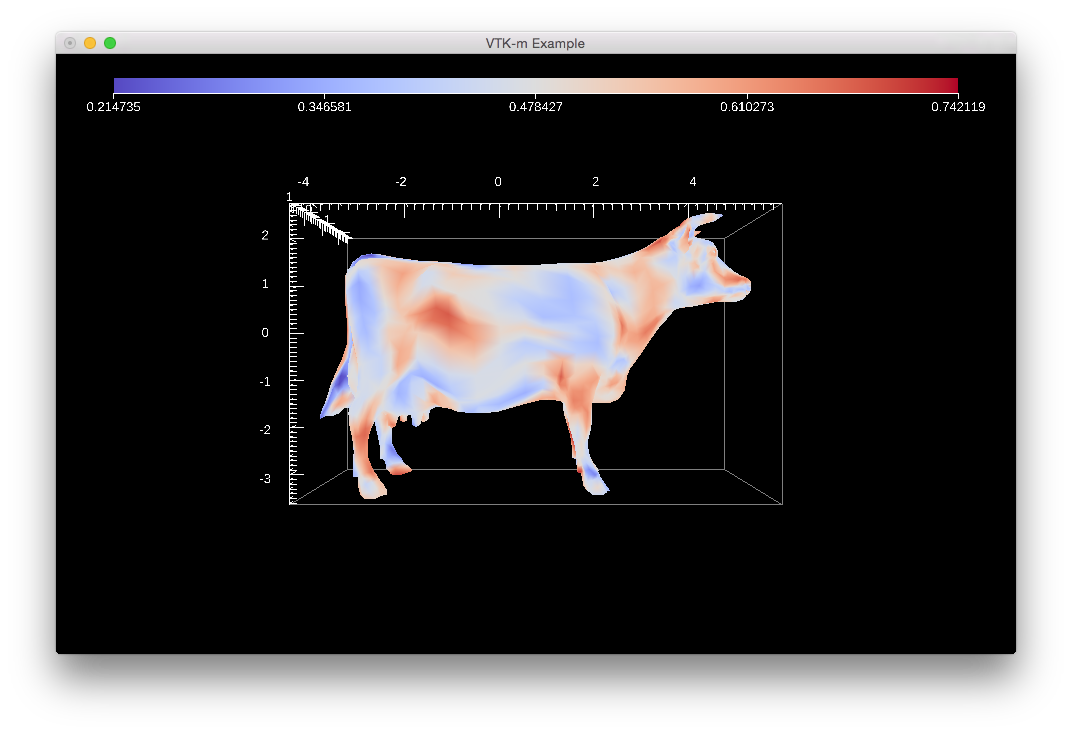
\includegraphics[width=4in]{images/BasicGlut}
  \caption{Output of the rendering program listed in
    Example~\ref{ex:BasicGlut}.}
  \label{fig:BasicGlut}
\end{figure}

\index{OpenGL|)}
\index{GLUT|)}
\index{canvas!OpenGL|)}
\index{canvas!GLUT|)}
\index{rendering!OpenGL|)}
\index{rendering!GLUT|)}

\subsection{Creating an Off Screen Rendering Canvas}

\index{rendering!off~screen|(}
\index{canvas!off~screen|(}
\index{off~screen|(}

Another use case for rendering in VTK-m is rendering to an off screen
buffer. This is the preferred method when doing automated visualization
such as when running visualization in situ with a simulation. VTK-m comes
built in with multiple methods to create off screen rendering contexts.
There are multiple subclasses to \vtkmrendering{Canvas} that, when
constructed, create their own rendering contexts, so can be used
immediately. All of these classes take as parameters to their constructors
the width and height of the image to create.

The following classes, when constructed, create an off screen rendering
buffer.

\begin{description}
\item[\vtkmrendering{CanvasOSMesa}] \index{rendering!OSMesa}
  \index{canvas!OSMesa} \index{OSMesa} Creates an off screen OpenGL
  rendering buffer using the OSMesa library. For this to be available,
  VTK-m must have been configured to use the OSMesa library. Also, be aware
  that OSMesa contexts do not use GPU hardware.
\item[\vtkmrendering{CanvasRayTracer}] \index{rendering!ray~tracing}
  \index{canvas!ray~tracing} \index{ray~tracing!canvas} Creates the frame
  buffers required for ray tracing. When invoking this canvas, you must use
  other ray tracing component where applicable. OpenGL rendering does not
  work with the \textidentifier{CanvasRayTracer}.
\end{description}

\index{canvas!off~screen!saving}
\index{off~screen!saving}

By their nature, when writing to an off screen canvas, you cannot directly
see the result. Typically, programs using off screen rendering save
rendered images as files to be viewed later. For convenience,
\textidentifier{Canvas} has a method named \textcode{SaveAs} that will
write the contents of the last saved image to a file. The files are written
in \index{portable~pixel~map}\index{PPM} portable pixel map (PPM) format,
which are also valid \index{portable~anymap~format}\index{PNM} portable
anymap format (PNM) files. This is a very simple format that is easy to
read and write. PPM files are supported by the
ImageMagick\footnote{\url{http://imagemagick.org}} software suite as well
as many other image software tools.

\vtkmlisting{Saving an image rendered in a \textidentifier{Canvas} to a file.}{SaveCanvasImage.cxx}

Alternately, the rendered image can be retrieved directly from the
\textidentifier{Canvas} by first calling the \textcode{RefreshColorBuffer}
method and then calling \textcode{GetColorBuffer}. This retrieves the raw
image data as a \vtkmcont{ArrayHandle}. \textidentifier{ArrayHandle}s are
documented later in Chapter~\ref{chap:ArrayHandle}.

\index{off~screen|)}
\index{canvas!off~screen|)}
\index{rendering!off~screen|)}

\index{canvas|)}
\index{rendering!canvas|)}


\section{Scenes and Actors}
\label{sec:Scene}
\label{sec:Actor}

\index{rendering!actor|(}
\index{actor|(}

The primary intent of the rendering package in VTK-m is to visually display
the data that is loaded and processed. Data are represented in VTK-m by
\vtkmcont{DataSet} objects. \textidentifier{DataSet} is presented in
Chapters \ref{chap:FileIO} and \ref{chap:ProvidedFilters}. For now we treat
\textidentifier{DataSet} mostly as an opaque object that can be passed
around readers, writers, filters, and rendering units. Detailed
documentation for \textidentifier{DataSet} is provided in
Chapter~\ref{chap:DataSet}.

To render a \textidentifier{DataSet}, the data are wrapped in a
\vtkmrendering{Actor} class. The \textidentifier{Actor} holds the
components of the \textidentifier{DataSet} to render (a cell set, a
coordinate system, and a field). A color table can also be optionally be
specified, but a default color table will be specified otherwise.

\index{actor|)}
\index{rendering!actor|)}

\index{rendering!scene|(}
\index{scene|(}

\textidentifier{Actor}s are collected together in an object called
\vtkmrendering{Scene}. An \textidentifier{Actor} is added to a
\textidentifier{Scene} with the \textcode{AddActor} method. The following
example demonstrates creating a \textidentifier{Scene} with one
\textidentifier{Actor}.

\index{scene|)}
\index{rendering!scene|)}

\vtkmlisting{Creating an \textidentifier{Actor} and adding it to a \textidentifier{Scene}.}{ActorScene.cxx}


\section{Mappers}
\label{sec:Mapper}

\index{rendering!mapper|(}
\index{mapper|(}

A \keyterm{mapper} is a unit that converts data (managed by an
\textidentifier{Actor}) and issues commands to the rendering subsystem to
generate images. All mappers in VTK-m are a subclass of
\vtkmrendering{Mapper}. Different rendering systems (as established by the
\textidentifier{Canvas}) often require different mappers. Also, different
mappers could render different types of data in different ways. For
example, one mapper might render polygonal surfaces whereas another might
render polyhedra as a translucent volume. Thus, a mapper should be picked
to match both the rendering system of the \textidentifier{Canvas} and the
data in the \textidentifier{Actor}.

The following mappers are provided by VTK-m.

\begin{description}
\item[\vtkmrendering{MapperGL}] Uses OpenGL to render surfaces. If the data
  contain polyhedra, then their faces are rendered.
  \textidentifier{MapperGL} only works in conjunction with
  \textidentifier{CanvasGL} or one of its subclasses.
\item[\vtkmrendering{MapperRayTracer}] Uses VTK-m's built in ray tracing
  system to render the visible surface of a mesh.
  \textidentifier{MapperRayTracer} only works in conjunction with
  \textidentifier{CanvasRayTracer}.
\item[\vtkmrendering{MapperVolume}] Uses VTK-m's built in ray tracing
  system to render polyhedra as a translucent volume.
  \textidentifier{MapperVolume} only works in conjunction with
  \textidentifier{CanvasRayTracer}.
\end{description}

\index{mapper|)}
\index{rendering!mapper|)}


\section{Views}

\index{rendering!view|(}
\index{view|(}

A \keyterm{view} is a unit that collects all the structures needed to
perform rendering. It contains everything needed to take a
\textidentifier{Scene} (Section~\ref{sec:Scene}) and use a
\textidentifier{Mapper} (Section~\ref{sec:Mapper}) to render it onto a
\textidentifier{Canvas} (Section~\ref{sec:Canvas}). The view also annotates
the image with spatial and scalar properties.

The base class for all views is \vtkmrendering{View}. \textidentifier{View}
is an abstract class, and you must choose one of the two provided
subclasses, \vtkmrendering{View3D} and \vtkmrendering{View2D}, depending on
the type of data being presented. (All three classes are defined in the
\vtkmheader{vtkm/rendering}{View.h} header file.) Both
\textidentifier{View3D} and \textidentifier{View2D} take a
\textidentifier{Scene}, a \textidentifier{Mapper}, and a
\textidentifier{Canvas} as arguments to their constructor.

\vtkmlisting[ex:ConstructView]{Constructing a \textidentifier{View}.}{ConstructView.cxx}

\index{color}
The \textidentifier{View} constructors also take an optional fourth
argument for the background color. The background color (like other colors)
is specified using the \vtkmrendering{Color} helper class, which manages
the red, green, and blue color channels as well as an optional alpha
channel. These channel values are given as floating point values between 0
and 1.

\vtkmlisting{Creating a \textidentifier{View} with a background color.}{ViewBackgroundColor.cxx}

Once the \textidentifier{View} is created but before it is used to render,
the \textcode{Initialize} method should be called. This is demonstrated in
Example~\ref{ex:ConstructView}.

Once the \textcode{Initialize} method is called, the \textidentifier{View}
is ready to render the scene. This happens by calling the \textcode{Paint}
method, which will render the data into the contained canvas. When using
GLUT, as in Example~\ref{ex:BasicGlut}, or with most other GUI-based
systems, \textcode{Paint} is called in the display callback.

\vtkmlisting{Using \textidentifier{Canvas}\textcode{::Paint} in a display callback.}{PaintView.cxx}

\index{view|)}
\index{rendering!view|)}


\section{Manipulating the Camera}

\index{rendering!camera|(}
\index{camera|(}

The \vtkmrendering{View} uses an object called \vtkmrendering{Camera} to
describe the vantage point from which to draw the geometry. The camera can
be retrieved from the \textidentifier{View}'s \textcode{GetCamera} method.
That retrieved camera can be directly manipulated or a new camera can be
provided by calling \textcode{SetCamera} on the \textidentifier{View}.

A \textidentifier{Camera} operates in one of two major modes: 2D mode or 3D
mode. 2D mode is designed for looking at flat geometry (or close to flat
geometry) that is parallel to the x-y plane. 3D mode provides the freedom
to place the camera anywhere in 3D space. The different modes can be set
with \textcode{SetModeTo2D} and \textcode{SetModeTo3D}, respectively. The
interaction with the camera in these two modes is very different.

\subsection{2D Camera Mode}

\index{rendering!camera!2D|(}
\index{camera!2D|(}

\subsubsection{View Range}

\index{rendering!camera!view~range|(}
\index{camera!view~range|(}

\fix{Do this}

\index{camera!view~range|)}
\index{rendering!camera!view~range|)}

\subsubsection{Pan}

\index{rendering!camera!pan|(}
\index{camera!pan|(}

\fix{Do this}

\index{camera!pan|)}
\index{rendering!camera!pan|)}

\subsubsection{Zoom}

\index{rendering!camera!zoom|(}
\index{camera!zoom|(}

\fix{Do this}

\index{camera!zoom|)}
\index{rendering!camera!zoom|)}

\index{camera!2D|)}
\index{rendering!camera!2D|)}

\subsection{3D Camera Mode}

\index{rendering!camera!3D|(}
\index{camera!3D|(}

\subsubsection{Position and Orientation}

\fix{ClippingRange}
\fix{Position}
\fix{LookAt (a.k.a. focal point)}
\fix{ViewUp}
\fix{FieldOfView}

\subsubsection{Movement}

\fix{Roll}
\fix{Azimuth}
\fix{Elevation}
\fix{Dolly}

\subsubsection{Pan}

\index{rendering!camera!pan|(}
\index{camera!pan|(}

\fix{Do this}

\index{camera!pan|)}
\index{rendering!camera!pan|)}

\subsubsection{Zoom}

\index{rendering!camera!zoom|(}
\index{camera!zoom|(}

\fix{Do this}
\fix{Note this is different than dolly}

\index{camera!zoom|)}
\index{rendering!camera!zoom|)}

\subsubsection{Interactive Rotations}

\index{rendering!camera!mouse|(}
\index{camera!mouse|(}
\index{mouse~rotation|(}

\fix{TrackballRotate}

\index{mouse~rotation|)}
\index{camera!mouse|)}
\index{rendering!camera!mouse|)}

\index{camera!3D|)}
\index{rendering!camera!3D|)}

\index{camera|)}
\index{rendering!camera|)}

\index{rendering|)}

\subsubsection{Reset}

\index{rendering!camera!reset|(}
\index{camera!reset|(}

\fix{ResetToBounds}
\fix{Add example to reset down axis}

\index{camera!reset|)}
\index{rendering!camera!reset|)}


\section{Color Tables}
\label{sec:ColorTables}

\index{rendering!color~tables|(}
\index{color~tables|(}

\index{color~tables|)}
\index{rendering!color~tables|)}
